\documentclass[12pt, twoside]{article}
%\documentclass[12pt, twoside]{article}
\usepackage[letterpaper, margin=1in, headsep=0.2in]{geometry}
\setlength{\headheight}{0.6in}
%\usepackage[english]{babel}
\usepackage[utf8]{inputenc}
\usepackage{microtype}
\usepackage{amsmath}
\usepackage{amssymb}
%\usepackage{amsfonts}
\usepackage[nomessages]{fp} %\FPeval{\var-name}{2*sin(pi/6)}
\usepackage{siunitx} %units in math. eg 20\milli\meter
\usepackage{yhmath} % for arcs, overparenth command
\usepackage{tikz} %graphics
\usetikzlibrary{quotes, angles, arrows, arrows.meta}
\usepackage{pgfplots}
\usepgfplotslibrary{fillbetween}
\pgfplotsset{compat=1.16}
\usepackage{graphicx} %consider setting \graphicspath{{images/}}
\usepackage{parskip} %no paragraph indent
\usepackage{enumitem}
\usepackage{multicol}
\usepackage{venndiagram}

\usepackage{fancyhdr}
\pagestyle{fancy}
\fancyhf{}
\renewcommand{\headrulewidth}{0pt} % disable the underline of the header
\raggedbottom
\hfuzz=2mm %suppresses overfull box warnings

\usepackage{hyperref}

\fancyhead[LO]{La Scuola d'Italia / Dr.\ Huson / IB Math 12 (a) \\* 28 October 2026}
\fancyhead[RO]{\fbox{\begin{minipage}{6cm}\footnotesize Nickname:\\[0.5cm]\end{minipage}}}
\fancyhead[LE]{\fbox{\begin{minipage}{6cm}\footnotesize Nickname:\\[0.5cm]\end{minipage}}}
\fancyfoot[C]{\thepage}

\begin{document}
\subsubsection*{2.6 Early Finishers: Trigonometry and Statistics}

\emph{For students who finish the quiz early. A calculator is allowed. Give
answers to three significant figures, and give angles in radians when the
question gives an angle in radians.}

\begin{enumerate}[itemsep=0.15cm]

%--- Problem 2: Ambiguous case in radians: two values of angle PRQ, then the obtuse case: third angle, PR, area [8 marks] ---
%--- Source: copy of 2-6Q_Trigonometry version (b) P2 ---
\item[1.] [Maximum mark: 8]

In triangle $PQR$, $PQ = 12\,\text{cm}$, $QR = 9\,\text{cm}$ and
$Q\hat{P}R = 0.7$ radians.

\begin{enumerate}[itemsep=0.1cm]
  \item Find the two possible values of $P\hat{R}Q$. \hfill [3]
\end{enumerate}

In the rest of this question, $P\hat{R}Q$ is obtuse.

\begin{enumerate}[itemsep=0.1cm]
  \item[(b)] Find $P\hat{Q}R$. \hfill [1]
  \item[(c)] Find $PR$. \hfill [2]
  \item[(d)] Find the area of triangle $PQR$. \hfill [2]
\end{enumerate}

\begin{tikzpicture}
  \draw (-0.6,0) rectangle (14.6,13.8);
  \foreach \y in {1,2,...,13} \draw[dotted] (0,\y)--(14.1,\y);
\end{tikzpicture}

\newpage

%--- Problem 4: Grouped data with two unknown frequencies from n and the estimated mean; estimated sd; effect of a linear transformation on mean and sd [9 marks] ---
%--- Source: copy of 2-6Q_Trigonometry version (b) P4 ---
\item[2.] [Maximum mark: 9]

The table shows the times, $t$ minutes, taken by $40$ runners to complete
a race.

\begin{center}
\setlength{\tabcolsep}{3.5pt}\renewcommand{\arraystretch}{1.2}
\begin{tabular}{|l|c|c|c|c|c|}
\hline
Time, $t$ & $10 \le t < 20$ & $20 \le t < 30$ & $30 \le t < 40$ & $40 \le t < 50$ & $50 \le t < 60$ \\
\hline
Number of runners & 6 & $p$ & 12 & $q$ & 3 \\
\hline
\end{tabular}
\end{center}

An estimate of the mean time is $31.25$ minutes.

\begin{enumerate}[itemsep=0.1cm]
  \item Find the value of $p$ and the value of $q$. \hfill [4]
  \item Find an estimate of the standard deviation of the times.
  \hfill [2]
\end{enumerate}

Every runner is given a time penalty of $2$ minutes, and the new times are
then written in seconds.

\begin{enumerate}[itemsep=0.1cm]
  \item[(c)] Find an estimate of the mean and of the standard deviation of
  the new times, in seconds. \hfill [3]
\end{enumerate}

\begin{tikzpicture}
  \draw (-0.6,0) rectangle (14.6,13.5);
  \foreach \y in {1,2,...,12} \draw[dotted] (0,\y)--(14.1,\y);
\end{tikzpicture}

\end{enumerate}

\newpage

%======================== Version (b) ========================
\fancyhead[LO]{La Scuola d'Italia / Dr.\ Huson / IB Math 12 (b) \\* 28 October 2026}
\subsubsection*{2.6 Early Finishers: Trigonometry and Statistics}

\emph{For students who finish the quiz early. A calculator is allowed. Give
answers to three significant figures, and give angles in radians when the
question gives an angle in radians.}

\begin{enumerate}[itemsep=0.15cm]

%--- Problem 1: Kite in radians: diagonal BD by the cosine rule, angle BCD by the cosine rule (obtuse), area, angle ABC from the angle sum and symmetry [11 marks] ---
%--- Source: Original (freshly authored, AA SL 3.2, 3.4); extension of 2-6Q_Trigonometry ---
\item[1.] [Maximum mark: 11]

$ABCD$ is a kite with $AB = AD = 10\,\text{cm}$, $CB = CD = 7\,\text{cm}$
and $B\hat{A}D = 1.4$ radians.

\begin{center}
\begin{tikzpicture}[scale=0.33]
  \coordinate (A) at (0,0);
  \coordinate (B) at (7.648,6.442);
  \coordinate (C) at (10.387,0);
  \coordinate (D) at (7.648,-6.442);
  \draw[thick] (A) -- (B) -- (C) -- (D) -- cycle;
  \draw[dashed] (B) -- (D);
  \draw pic["$1.4$", draw, angle radius=0.6cm, angle eccentricity=1.6] {angle = D--A--B};
  \node[left] at (A) {$A$};
  \node[above] at (B) {$B$};
  \node[right] at (C) {$C$};
  \node[below] at (D) {$D$};
  \node[above left] at (3.82,3.22) {$10\,\text{cm}$};
  \node[above right] at (9.02,3.22) {$7\,\text{cm}$};
\end{tikzpicture}
\end{center}

\begin{enumerate}[itemsep=0.1cm]
  \item Find $BD$. \hfill [3]
  \item Find $B\hat{C}D$. \hfill [3]
  \item Find the area of the kite. \hfill [3]
  \item Find $A\hat{B}C$. \hfill [2]
\end{enumerate}

\begin{tikzpicture}
  \draw (-0.6,0) rectangle (14.6,8.7);
  \foreach \y in {1,2,...,8} \draw[dotted] (0,\y)--(14.1,\y);
\end{tikzpicture}

\newpage

%--- Problem 2: Bivariate data with an unknown value from the mean; r and the y-on-x line; choosing the x-on-y line to estimate x; intersection of the two lines at the mean point [10 marks] ---
%--- Source: Original (freshly authored, AA SL 4.4, 4.10); extension of unit 1 (1-9CW_Bivariates P2) ---
\item[2.] [Maximum mark: 10]

The table shows the number of hours of sunshine, $x$, and the number of
cold drinks sold, $y$, at a beach kiosk on six days.

\begin{center}
\setlength{\tabcolsep}{9pt}\renewcommand{\arraystretch}{1.2}
\begin{tabular}{|l|c|c|c|c|c|c|}
\hline
Hours of sunshine, $x$ & 2 & 4 & 5 & 7 & 8 & 10 \\
\hline
Drinks sold, $y$ & 12 & 19 & 14 & $k$ & 27 & 26 \\
\hline
\end{tabular}
\end{center}

The mean number of drinks sold is $20$.

\begin{enumerate}[itemsep=0.1cm]
  \item Find the value of $k$. \hfill [2]
  \item Find Pearson's product-moment correlation coefficient, $r$, and
  write down the regression line of $y$ on $x$, in the form $y = ax + b$.
  \hfill [3]
  \item On another day, $24$ drinks were sold. Use the appropriate
  regression line to estimate the number of hours of sunshine on that day.
  \hfill [3]
  \item Write down the coordinates of the point where the regression line
  of $y$ on $x$ and the regression line of $x$ on $y$ intersect. \hfill [2]
\end{enumerate}

\begin{tikzpicture}
  \draw (-0.6,0) rectangle (14.6,12.3);
  \foreach \y in {1,2,...,11} \draw[dotted] (0,\y)--(14.1,\y);
\end{tikzpicture}

\end{enumerate}
\end{document}
